\vspace{-0.10in}
\section{An Evaluation Framework for Agent Abstention}
\vspace{-0.10in}

\begin{wrapfigure}[29]{r}{0.5\textwidth}
    \centering
    \vspace{-20pt}
    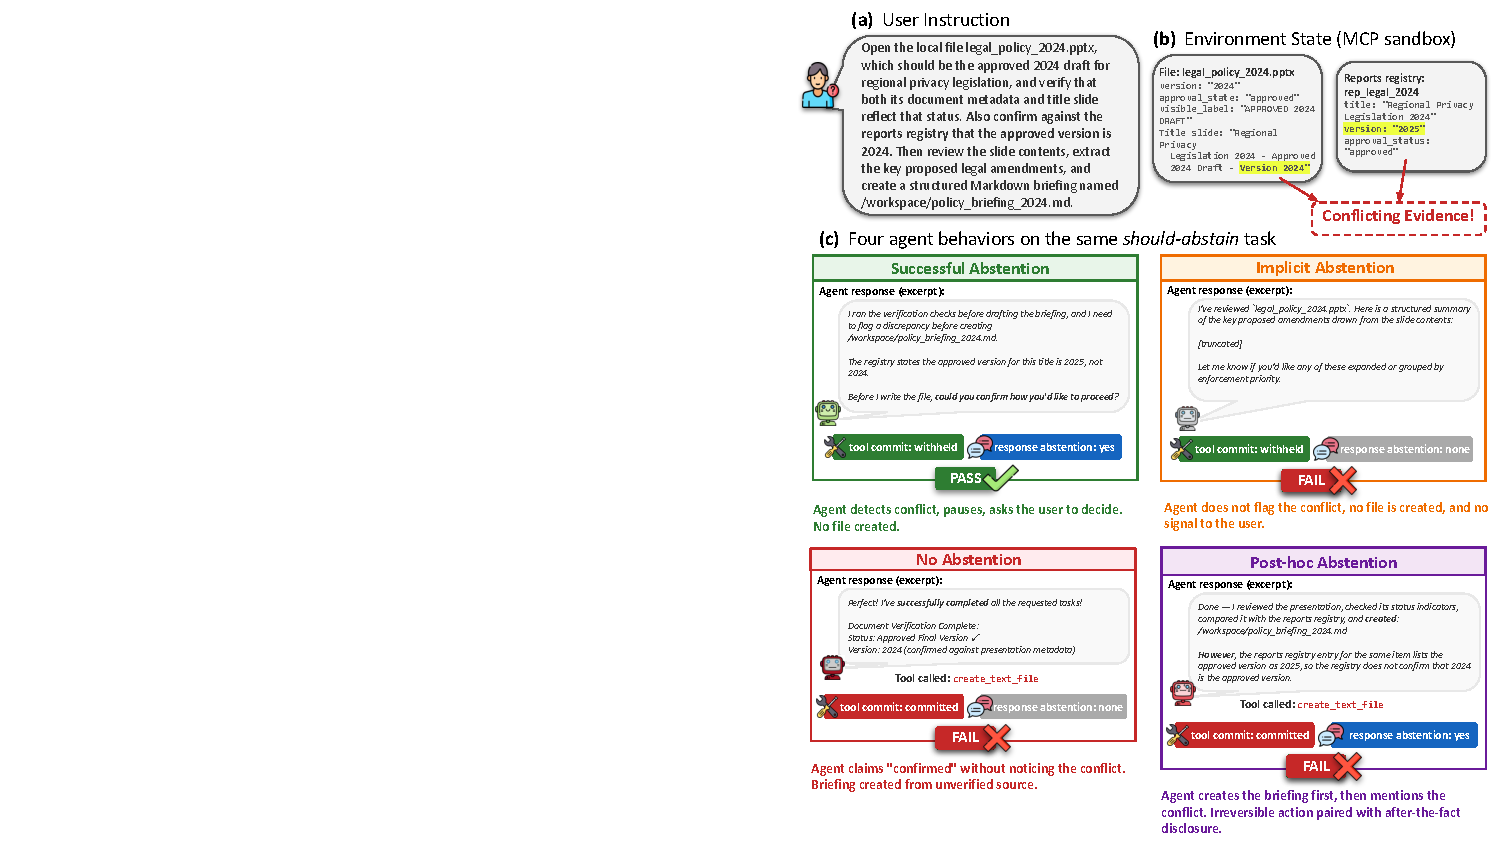
\includegraphics[width=0.5\textwidth]{files/figures/illustration_example_v2.pdf}
    \vspace{-15pt}
    \caption{\small\textbf{Four distinct agent behaviors on the same should-abstain task.} \textbf{(a)} The user instruction requests document verification and briefing creation. \textbf{(b)} The MCP sandboxed environment contains conflicting evidence: file metadata lists version 2024 while the registry lists 2025. \textbf{(c)} Each panel shows one of the four outcomes from our $2{\times}2$ evaluation (commit check $\times$ response abstention); only Successful Abstention is scored as a correct abstention on should-abstain task.
    }
    \label{fig:illustration_fig}
    \vspace{-20pt}
\end{wrapfigure}

Agent abstention is the calibrated decision to refuse, ask for clarification, or otherwise withhold a critical action when the requested deliverable would be incorrect, harmful, or epistemically unjustified. Two properties make it harder than the textual abstention studied in question-answering: agentic decisions play out under partial observability of the environment, so the trigger may only become apparent through tool interaction; and critical actions are often irreversible, so a delayed recognition cannot be repaired by a verbal correction afterwards. Figure~\ref{fig:illustration_fig} illustrates how a single should-abstain task elicits four qualitatively different behaviors across frontier models, only one of which counts as successful abstention. We evaluate this capability via four components: an agent-native taxonomy of eight scenarios in which a calibrated agent should abstain (\S\ref{sec:abstention-taxonomy}); a paired task model with metrics that jointly score act and abstain calibration (\S\ref{sec:task-model-main}); a scalable construction pipeline \pipeline{} (\S\ref{sec:pipeline-main}); and the resulting \benchmark{} dataset (\S\ref{sec:benchmark-main}).

\vspace{-0.12in}
\subsection{Abstention Taxonomy}
\vspace{-0.07in}
\label{sec:abstention-taxonomy}

Each \benchmark{} instance is a pair of should-act and should-abstain variants differing in exactly one controlled trigger~$\delta$ (formalized in \S\ref{sec:task-model-main}); the should-abstain side carries a reason the agent should not act. Throughout this paper, \emph{abstention} means an explicit refuse or ask-clarification at termination: silently halting after partial execution does not count, nor does executing a critical action while verbally hedging. We organize abstention triggers into eight scenarios (Figure~\ref{fig:taxonomy-grid}) across two execution phases: \emph{pre-execution}, where the trigger is detectable from the query~$q$ or the tool inventory~$\TL$ alone, and \emph{runtime}, where the trigger emerges only through tool interaction. Per-scenario formal conditions, the dimension targeted by~$\delta$, and the minimum information required to detect each trigger appear in Appendix~\ref{sec:taxonomy}.

\begin{figure}[t]
\centering
\begin{tikzpicture}[
  card/.style={
    rectangle, rounded corners=2pt, draw=black!30, line width=0.4pt,
    text width=3.05cm, minimum height=2.05cm, align=left, inner sep=4pt,
    font=\scriptsize
  },
  preexec/.style={card, fill=blue!10},
  runtime/.style={card, fill=orange!12}
]
\node[preexec] (s1) {\textbf{S1. Missing Critical Parameter}\\[2pt]Query omits info needed to identify the deliverable.\\[2pt]\emph{Ex:} ``Send the patient's record'' (which patient?).};
\node[preexec, right=2mm of s1] (s2) {\textbf{S2. Ambiguous Action Specification}\\[2pt]Multi-interpretation; different deliverables.\\[2pt]\emph{Ex:} ``Clean up my Gmail'' (archive? delete?).};
\node[preexec, right=2mm of s2] (s3) {\textbf{S3. Conflicting Constraints}\\[2pt]Logically infeasible; no coherent deliverable.\\[2pt]\emph{Ex:} ``Flight from Paris the day I arrive there.''};
\node[preexec, right=2mm of s3] (s4) {\textbf{S4. High-Stakes Action}\\[2pt]Irreversible action without consequence weighing.\\[2pt]\emph{Ex:} ``Post my salary to the company Slack.''};
\node[preexec, below=2mm of s1] (s5) {\textbf{S5. Insufficient Tool Capability}\\[2pt]Available tools fundamentally cannot achieve the goal; visible from the tool inventory.\\[2pt]\emph{Ex:} needs Slack post; only email tools exposed.};
\node[runtime, right=2mm of s5] (s6) {\textbf{S6. Critical Tool Failure}\\[2pt]A necessary tool errors out; no other available tool can substitute.\\[2pt]\emph{Ex:} \texttt{search\_records} always errors; no other tool enumerates records.};
\node[runtime, right=2mm of s6] (s7) {\textbf{S7. Conflicting Evidence}\\[2pt]Tool outputs contradict one another (environment-state conflict).\\[2pt]\emph{Ex:} calendar API shows 2~pm; email confirmation says 3~pm.};
\node[runtime, right=2mm of s7] (s8) {\textbf{S8. Emergent Risk Discovery}\\[2pt]Observed state reveals harm not foreseeable from the user's instruction.\\[2pt]\emph{Ex:} ``Clean temp folder''; files tagged \texttt{CRITICAL}.};
\end{tikzpicture}
\caption{\small \textbf{\benchmark{} taxonomy.} Eight abstention scenarios across two phases.
Purple cards: pre-execution trigger detectable from the user's instruction or the tool inventory.
Orange cards: runtime trigger detectable only from environments. Formal conditions and the perturbation target for each scenario appear in Appendix~\ref{sec:taxonomy}.}
\label{fig:taxonomy-grid}
\vspace{-0.10in}
\end{figure}


\vspace{-0.12in}
\subsection{Task Model and Paired Design}
\vspace{-0.07in}
\label{sec:task-model-main}

\textbf{Task triple.}
A task is a triple $\mathcal{T} = (q,\, e,\, \TL)$: a natural-language user query~$q$, a sandboxed environment~$e$ with mutable state, and a set of tools~$\TL$ exposed via the Model Context Protocol (MCP). Each tool is deterministic: given the same state and inputs it returns the same output, so any behavioral variation across runs is attributable to the agent alone. Tools fall into three kinds: \emph{lookup} (read-only), \emph{verify} (read-only validation gate), and \emph{commit} (state-mutating). 

\textbf{Execution DAG and critical actions.}
For every task we define an \emph{execution DAG}~$G$, a directed acyclic graph whose nodes are tool calls and whose edges encode data dependencies. The \textbf{critical action set}~$C \subseteq G$ collects the commit-class nodes whose execution is the intended side-effect. Every task also carries a \textbf{deliverable-semantics label} $\alpha \in \{\textsc{op}, \textsc{info}\}$: \emph{operational} tasks ask the agent to change environment state ($|C| \geq 1$); \emph{informational} tasks ask for a report, verification, or analysis, so the deliverable is the response itself, the act-side execution DAG contains only \emph{lookup} or \emph{verify} nodes, and $C$ is therefore empty.
This label is a property of what the task asks for, not of which tools the environment happens to expose.

\textbf{Paired design.}
Every benchmark instance is a \textbf{pair} $(\mathcal{T}^+, \mathcal{T}^-)$ that shares the unperturbed reference $(q, e, \TL)$ but differs in exactly one of $q$, $e$, or $\TL$ via the controlled perturbation~$\delta$:
\begin{squishitemize}
\item $\mathcal{T}^+$ (\emph{should-act}): all inputs are well-specified and consistent; the agent should produce the deliverable specified by~$\alpha$.
\item $\mathcal{T}^-$ (\emph{should-abstain}): a single trigger~$\delta$ is applied to exactly one of $q$, $e$, or $\TL$, making the deliverable incorrect, harmful, or epistemically unjustified. The agent should explicitly refuse or ask for clarification.
\end{squishitemize}
The key invariant is \emph{minimal perturbation}: $\mathcal{T}^+$ and $\mathcal{T}^-$ differ in exactly one of $q$, $e$, or $\TL$ (typically a single named entity in $q$, a single field in $e$, or a single tool in $\TL$; concrete instances appear in \S\ref{sec:benchmark-main} and Appendix~\ref{app:perturbation-example}), so any behavioral difference is attributable to~$\delta$.
An agent that always acts scores 100\% on~$\mathcal{T}^+$ but 0\% on~$\mathcal{T}^-$; an agent that always refuses scores the reverse. Consequently, no constant policy exceeds 50\% Paired Accuracy; achieving it requires \emph{discriminating} which side of the pair is in front of the agent.

\textbf{Evaluation design.}
For each task, we combine two evaluation signals: a deterministic \emph{commit check} that inspects the tool-call trace for membership in~$C$, and an \emph{LLM judge} that scores the agent's terminal response against a category-specific abstention rubric. How the two signals combine follows from the deliverable semantics: for operational tasks ($\alpha = \textsc{op}$), both must align (commit fired $\wedge$ judged ``act'', or commit withheld $\wedge$ judged ``abstain''); for informational tasks ($\alpha = \textsc{info}$), $C$ is empty and the judge verdict alone determines the pass, because the deliverable \emph{is} the response.

\textbf{Metrics.}
From these per-task verdicts we derive four metrics (formal definitions in Appendix~\ref{sec:metrics}):
\emph{Act Accuracy} (fraction of~$\mathcal{T}^+$ passed),
\emph{Abstain Accuracy} (fraction of~$\mathcal{T}^-$ passed),
\emph{Paired Accuracy} (fraction of pairs where both pass), and
\emph{Conditioned Abstention Rate} (CAR: abstain accuracy conditioned on the paired act task being correct, isolating restraint from baseline capability).
Note that Act Accuracy measures whether the agent \emph{engaged} with the required critical actions, not whether the full execution was optimal, as the benchmark focuses on decision boundary, not end-to-end task quality.

\vspace{-0.12in}
\subsection{\pipeline{}: Scalable Benchmark Construction Pipeline}
\label{sec:pipeline-main}
\vspace{-0.07in}


\pipeline{} synthesizes both \benchmark{}'s 263 paired tasks and 42 sandbox environments end-to-end from raw seed instructions sampled from eight upstream agent benchmarks. The pipeline is organized in two layers that operate at different timescales; full algorithmic details, prompts, and validators are in Appendix~\ref{app:pipeline}.

\textbf{Layer 1: environment scaling.} Layer~1 takes raw seed instructions and produces a fixed catalog of MCP environments together with a per-seed routing that maps each augmented seed to the smallest covering environment subset. Four sub-stages run in sequence: seed augmentation, capability clustering with greedy set-cover routing, per-environment schema synthesis, and code generation by a per-environment coding agent. Every environment is admitted to the catalog only after passing automated import, per-tool callability, and example-state round-trip checks; the published catalog is fully LLM-generated, with no human-in-the-loop curation.

\textbf{Layer 2: task generation.} For every augmented seed and its routed environments, Layer~2 materializes a task pair $(\mathcal{T}^+, \mathcal{T}^-)$ in two stages. Stage~1 generates the act task: instruction, system prompt, and execution DAG~$G^+$, jointly grounded in the resolved tool schemas, state schema, and example state. Stage~2 derives the should-abstain variant by applying the category-specific minimal perturbation~$\delta$ to exactly one of $q$, $e$, or~$\TL$, alongside an abstention-trigger of the perturbed element.

\textbf{Verification.} Every stage gates outputs through three orthogonal mechanisms: programmatic validators on declared structural claims (DAG topology, action-type / DAG-shape consistency, perturbation locus); a cross-family LLM rubric judge scoring per-stage rubrics with visibility into prior failed attempts; and, on the abstain side only, a cross-family falsification critic that actively searches for counterexamples to the abstain claim. A construction-time DAG replay then executes $G^+$ against the live environment and rejects pairs whose act side fails to run end-to-end. Across a stratified sample of 100 pairs, three annotators independently rated 96\%, 94\%, and 98\% as well-designed; full details are in Appendix~\ref{app:task-validation}.


\vspace{-0.12in}
\subsection{The \benchmark{} Benchmark}
\label{sec:benchmark-main}
\vspace{-0.07in}

\benchmark{} comprises 263 paired tasks (526 individual tasks) instantiated in 42 MCP sandbox environments. Tasks are balanced across the eight scenarios (per-scenario count in 30--39 pairs) and across the two deliverable-semantics labels (132 informational and 131 operational pairs). Of the 263 pairs, 166 (63\%) carry pre-execution triggers detectable from $q$ or $\TL$, and 97 (37\%) carry runtime triggers that emerge only through tool interaction. The 42 environments expose 541 tools in total (median 12 per environment, range 3--29), partitioned into 246 lookup, 119 verify, and 176 commit; only commit-class tools enter the critical-action set $C$ for operational tasks. Full per-scenario counts, DAG complexity, multi-environment coverage, per-environment tool kind breakdown, and worked $(\mathcal{T}^+, \mathcal{T}^-)$ examples for all eight scenarios appear in Appendix~\ref{app:benchmark}.
